\documentclass[12pt]{article}

\usepackage{fontawesome}
\usepackage{hyperref}
\usepackage{xurl}
\usepackage{graphicx}
\usepackage{float}
\usepackage[tagged, highstructure]{accessibility}
\usepackage{bookmark}
\usepackage{enumitem}

\hypersetup{
    colorlinks=false,
    pdfborder={0 0 0},
    pdftitle={Cloud Security},
    pdfauthor={Adrianna Holden-Gouveia},
    pdfsubject={Information Security - Lab Assignment},
    pdflang={en-US},
    pdfkeywords={cloud security, SaaS, privacy policy, cloud outage, AWS}
}

% Configure PDF bookmarks for navigation
\bookmarksetup{
    numbered,
    open,
}

% Configure list spacing for better accessibility
\setlist{nosep}



\title{Cloud Security}
\author{
        Adrianna Holden-Gouveia \\
        Website: \href{https://aholdengouveia.name}{aholdengouveia.name}\\ 
        \date{\vspace{-5ex}}
        %Email: \href{mailto:admin@aholdengouveia.name}{admin@aholdengouveia.name} \\
%        \faLinkedin{: aholdengouveia} \\
        \faGithub {: aholdengouveia} \\
        \faTwitter {: aholdengouveia} \\
        }

%S\date{\today}


\begin{document}

\maketitle

\section*{Accessibility Notice}
This document is also available in HTML format at:

Link: \href{https://aholdengouveia.name/InfoSec/labs/cloudsecurity.html}{\textbf{\nolinkurl{https://aholdengouveia.name/InfoSec/labs/cloudsecurity.html}}}

The HTML version provides enhanced accessibility features including keyboard navigation, screen reader support, responsive design, dark mode support, and high contrast options.

\section*{Learning Outcomes}
By the end of this lab, you will be able to:
\begin{itemize}
    \item Identify the cloud services you use, and classify them by service model
    \item Evaluate who can access your data in the cloud, using privacy policies and account settings
    \item Explain how a cloud outage affects the people and businesses that depend on it
    \item Plan how to keep going if a cloud service you rely on goes down
\end{itemize}

\section*{Lab Instructions}
Most of your data probably lives in the cloud: photos, email, schoolwork, and games. In this lab, you'll look at the cloud services you use, check who can get to your data, and see what happens when the cloud goes down.

\subsection*{Screenshots}
This lab asks for about 6 screenshots. Each screenshot should have your name, term, and year.  One of the easiest ways to do that is make a text document with your name and term/year on your computer and save it to use all term. Any screenshots that don't include this information won't be counted.

\begin{figure}[H]
    \centerline{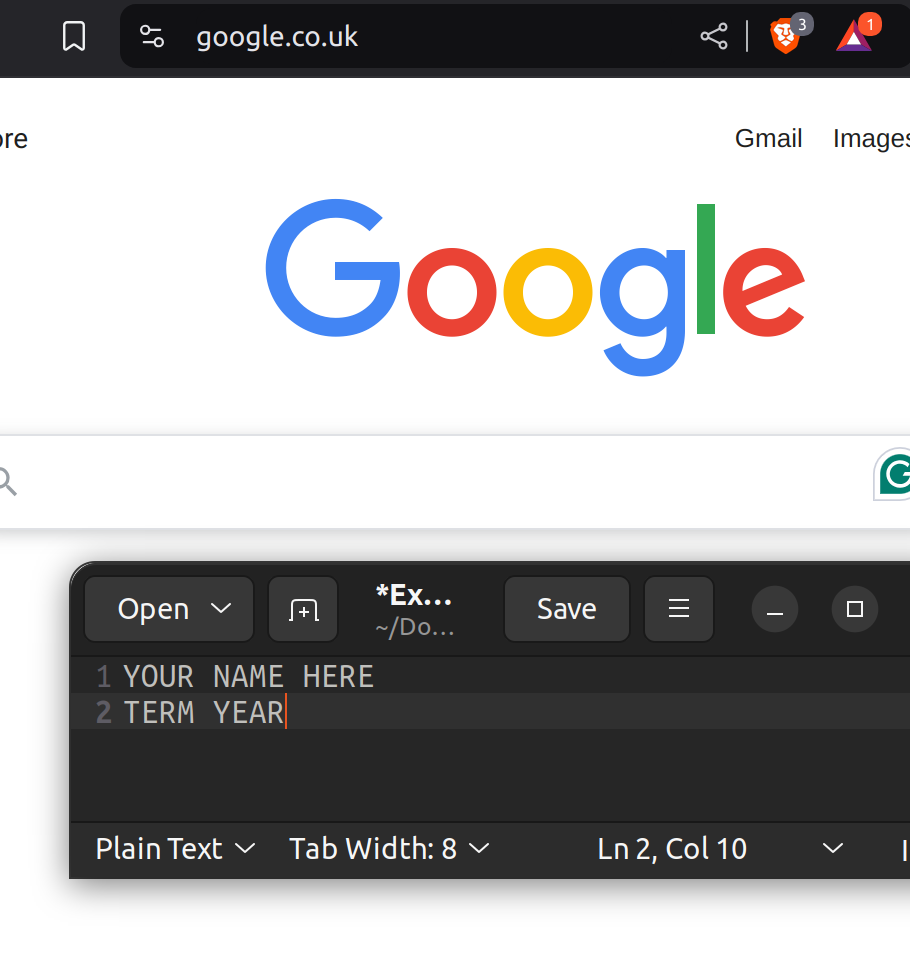
\includegraphics[scale=.2]{ExampleScreenshot.png}}
    \caption{This is an image of what each of your screenshots should look like}
    \alt{Example screenshot: a web browser showing the Google home page, with a small text editor window in front of it that says YOUR NAME HERE and TERM YEAR}
\end{figure}

\textbf{Blur or cover anything sensitive before you turn in a screenshot}, as long as your name and term note still shows. That includes email addresses, phone numbers, device names that include someone's name, and locations.

\subsection*{Part 1: Your Cloud}
\begin{enumerate}
    \item Make a table of 2 to 6 cloud services you use. Your school email and accounts count. Other examples: iCloud or Google Photos backup, Google Drive or OneDrive, Snapchat, Instagram, TikTok, Discord, Spotify, Netflix, Steam, or your Xbox, PlayStation, or Nintendo account. For each one, include:
    \begin{itemize}
        \item The service, and the company that runs it
        \item What you keep there
        \item Its service model: Software as a Service (SaaS), Platform as a Service (PaaS), or Infrastructure as a Service (IaaS). Almost every app you use is SaaS. PaaS and IaaS are mostly used by companies building their own apps, but you should still know the difference.
        \item Whether it's a public cloud, which many customers share, or a private cloud, used by one organization, such as a system your school runs itself
    \end{itemize}
    \item Which service would hurt the most to lose? Why?
\end{enumerate}
If you don't use any cloud services besides your school accounts, email me, and I'll give you another option.

\subsection*{Part 2: Who Can Get to Your Data?}
Pick 2 services from your table. One of them can be your school account. If you only have one service, email me for another option. For each one:
\begin{enumerate}[start=3]
    \item Find its privacy policy. Quote one thing it says about who can see or get your data, such as employees, other companies, or law enforcement.
    \item Quote what it says about encryption. Is your data encrypted while it's stored, and is it end-to-end encrypted, so even the company can't read it? If the policy doesn't say, write ``not stated''.
    \item Find the list of devices or sessions signed in to your account. Take a screenshot. Do you recognize all of them? If not, sign them out.
    \item Check whether two-factor authentication is turned on. Take a screenshot. If it's off, turn it on, if the service has it.
    \item Request a copy of your data, such as Google Takeout, Apple's Data and Privacy page, or the service's ``download your data'' option. Take a screenshot of the request. You don't need to download the whole thing.
    \item What surprised you most about these 2 services?
\end{enumerate}

\subsection*{Part 3: When the Cloud Goes Down}
On October 20, 2025, a problem in Amazon Web Services (AWS) took down thousands of apps and websites. Read Amazon's own summary of what happened, and one of the news articles, all linked under Resources.
\begin{enumerate}[start=9]
    \item In your own words, what caused the outage, and how long did it last?
    \item Name 3 apps or websites that went down. Do you use any of them, or did it affect you or someone you know?
    \item None of those apps were run by Amazon, but they went down anyway. Explain why. What does ``when you rely on one cloud provider, its outage is your outage'' mean?
    \item Find the status page for one cloud service you use, such as Discord's status page, your school's IT status page, or the service's page on Downdetector, a website where people report outages. Search for the service's name and ``status'' if you need to. Take a screenshot. Is everything working right now?
\end{enumerate}

\subsection*{Part 4: Your Backup Plan}
\begin{enumerate}[start=13]
    \item For the service you said would hurt most to lose in question 2, write a short plan. What would you do if it went down for a day? What if it disappeared for good? Include where you'd keep a second copy of your data, how you'd get to it offline, and how you'd reach people without it.
\end{enumerate}

\section*{Deliverables}
One file that includes:
\begin{itemize}
    \item Part 1: your table, and your answer
    \item Part 2: for each of your 2 services, your quotes, your 3 screenshots, and your answers
    \item Part 3: your answers, and your status page screenshot
    \item Part 4: your plan
\end{itemize}
Remember to blur sensitive information in every screenshot.

\section*{Resources}
References, a video, a PowerPoint and some notes are available at my website
Link: \href{https://www.aholdengouveia.name/InfoSec/CloudSecurity.html}{\textbf{\nolinkurl{https://www.aholdengouveia.name/InfoSec/CloudSecurity.html}}}

NIST's definition of cloud computing, including SaaS, PaaS, and IaaS
Link: \href{https://csrc.nist.gov/pubs/sp/800/145/final}{\textbf{\nolinkurl{https://csrc.nist.gov/pubs/sp/800/145/final}}}

Amazon's summary of the October 2025 AWS outage, for Part 3
Link: \href{https://aws.amazon.com/message/101925/}{\textbf{\nolinkurl{https://aws.amazon.com/message/101925/}}}

NPR: Outage at Amazon Web Services disrupts websites across the internet (2025), for Part 3
Link: \href{https://www.npr.org/2025/10/20/nx-s1-5580312/aws-outage}{\textbf{\nolinkurl{https://www.npr.org/2025/10/20/nx-s1-5580312/aws-outage}}}

PBS News: What to know about the Amazon Web Services outage (2025), for Part 3
Link: \href{https://www.pbs.org/newshour/world/what-to-know-about-the-amazon-web-services-outage}{\textbf{\nolinkurl{https://www.pbs.org/newshour/world/what-to-know-about-the-amazon-web-services-outage}}}

Google Takeout, to download your Google data
Link: \href{https://takeout.google.com/}{\textbf{\nolinkurl{https://takeout.google.com/}}}

Apple Data and Privacy, to download your Apple data
Link: \href{https://privacy.apple.com/}{\textbf{\nolinkurl{https://privacy.apple.com/}}}

Discord's status page, an example of a cloud status page
Link: \href{https://discordstatus.com/}{\textbf{\nolinkurl{https://discordstatus.com/}}}

Downdetector, where people report outages for apps and websites
Link: \href{https://downdetector.com/}{\textbf{\nolinkurl{https://downdetector.com/}}}

\end{document}
